\documentclass[a4paper]{article}

%% Language and font encodings
\usepackage[english]{babel}
\usepackage[utf8x]{inputenc}
\usepackage[T1]{fontenc}

%% Sets page size and margins
\usepackage[a4paper,top=3cm,bottom=2cm,left=3cm,right=3cm,marginparwidth=1.75cm]{geometry}

%% Useful packages
\usepackage{amsmath}
\usepackage{graphicx}
\usepackage{caption}
\usepackage{subcaption}
\usepackage{float}
\usepackage[colorinlistoftodos]{todonotes}
\usepackage[colorlinks=true, allcolors=blue]{hyperref}
%% package for Python code display from https://www.overleaf.com/9258172ycyrrgqnppgf
\usepackage{listings}
\usepackage{color}

\definecolor{mygreen}{rgb}{0,0.6,0}
\definecolor{mygray}{rgb}{0.5,0.5,0.5}
\definecolor{mymauve}{rgb}{0.58,0,0.82}
\definecolor{mycom}{RGB}{173,173,173}
\definecolor{mygr}{RGB}{0,170,0}

\lstset{ %
  backgroundcolor=\color{white},   % choose the background color
  basicstyle=\footnotesize,        % size of fonts used for the code
  breaklines=true,                 % automatic line breaking only at whitespace
  captionpos=b,                    % sets the caption-position to bottom
  commentstyle=\color{mycom},    % comment style
  escapeinside={\%*}{*)},          % if you want to add LaTeX within your code
  keywordstyle=\color{blue},       % keyword style
  stringstyle=\color{mygr},     % string literal style
}



\title{Influence of water vapour on autoignition of air-methane mixtures}
\author{Łukasz Osiński}

\begin{document}
\maketitle

\begin{abstract}
A reactor with a volume of 20 liters was set up using Cantera in Python. Maximal temperatures, pressures and maximal pressure rise were calculated as a function of initial methane volume fraction, temperature and pressure. Calculations were performed for three molar fractions of water in the mixture (0, 15.97\% and 27.54\%). Maximum rate of pressure rise was too far away from experimental data to be taken into consideration.
\end{abstract}

\section{Mathematical model}
Mixture consisting of: 1 mole air (defined as $78\%\ N_2\ 21\%\ O_2$ and $1\%Ar$), $ch4\_mol$ moles of $CH_4$ and $water\_mol$ moles of $H_2o$ was set up in a Cantera reactor with a volume of $20 l$. Autoignition process occurs and explosion maximum pressures (defined as $maximal\ pressure\ -\ initial\ pressure\ in\ the\ reactor$) and temperatures are calculated. Maximum rate of pressure rise was also calculated but the results were too far away from experimental data.

Calculations were performed for three molar fractions of water in the mixture: 0, 1 and 2 moles, (coresponding to 0\%, 15.97\% and 27.54\% of water vapour vol. in the mixture respectively).

\section{Python 3.6 program code}
\subsection{Preparing the program}
Necessary modules are imported.
\begin{lstlisting}[language=python]
import csv
import cantera as ct
import numpy as np
import matplotlib.pyplot as plt
\end{lstlisting}
\subsection{Creating the 'airm' function}
\subsubsection{Preparing the function}
Next a function $airm$ was created. It would take initial temperature $(temp)$ in K, initial pressure $(pressure)$ in Pa, $H_2O$ mole fraction $(water\_mol)$ and $CH_4$ mole fraction $(ch4\_mol)$ as arguments. Additionally $plot$ could be set to either $0, 1$ or $2$ for printing information abut the simulation to the console to a different extent of details.


	\begin{lstlisting}[language=python]
def airm(temp, pressure, water_mol, ch4_mol, plot):

\end{lstlisting}
    
This part of code is calculating stoichiometric conditions and allowing to set up $CH_4$ and $H_2O$ mole fractions

\begin{lstlisting}[language=python]
    #Calculating stoichiometry
    n2=0.78/0.21
    ar=0.01/0.21
    d="CH4:"+str(ch4_mol)+", O2:1, N2:"+str(n2)+", AR:"+str(ar)+", H2O:"+str(water_mol) 

    print (d+"\n") #Printing state of the gas to be set to the console
\end{lstlisting}
Creating mixture to autoignite
\begin{lstlisting}[language=python]
    gas = ct.Solution('gri30.xml')
    gas.TPX = temp, pressure, d #setting gas temperature as 'temp', pressure as 'pressure' and molar fractions as in 'd'
    gas.name = "Methane-air-water mixture"
    if plot==2: #additional information about the mixture to be printed if 'plot' was set to '2'
        print (gas())
    
    #Creating a reactor, filled up with 'gas' and with a volume of 0.02 cubic meters
    r = ct.Reactor(contents=gas, name='reactor', volume=0.02)
    
    print ('Water mass fraction = %10.3f %%\n' % (r.thermo['H2O'].Y*100))
    print ('Stoichiometry  index (phi) = %10.3f\n' % ((r.thermo['CH4'].X/r.thermo['O2'].X)/(0.5)) )
\end{lstlisting}
\subsubsection{Preparing simulation}
\begin{lstlisting}[language=python]
    #Preparing space for data 
    times = np.zeros(size)
    data = np.zeros((size,7))   
    time = 0.0 #starting time
    counter=size #setting 'counter' to 'size' (number of the loop iterations)
    #different basic time steps for differnet initial temperatures
    if temp>1400:
        current_step = 1.e-5 #shorter timestep for high temperatures
    elif temp>1100:
        current_step = 1.e-4 #shorter timestep for high temperatures
    else:
        current_step = 1.e-2 #basic time step
    dP=0
    
    f=open('data.txt', 'a') #preparing file for appending data
    
    sim = ct.ReactorNet([r]) #simulation
    size=20000 #number of iterations in the simulation advancing loop
    stepchange=0
    #different shorter time steps for different initial temperatures
    if temp>1400:
        short_step=1.e-6
    elif temp>1100:
        short_step=2.5*1.e-6
    else:
        short_step=1.e-4 #shorter time step [s] 
        
    itafex=((1.e-1)/short_step) #going through this many iterations at specified 
    #timestep='short_step' should be equal to advancing the simulation by 0.1 seconds
    print('%10s %10s %10s %14s' % ('t [s]','T [K]','P [Pa]','u [J/kg]'))    
    f.write("Initial temperature is %10.3f\n\n" % (temp))
    f.write ('%10s %10s %10s %10s %10s %10s %10s %10s' % ('t [s]','step [s]','dT [K]','T [K]', 'dP [Pa]', 'P [Pa]', 'licznik', 'iteration\n'))
\end{lstlisting}

\subsubsection{Advancing simulation}
The simulation is then advanced in a loop
\begin{lstlisting}[language=python]
    for n in range(size):
        time+= current_step
        sim.advance(time)
\end{lstlisting}
Data is stored in $times$ and $data$ arrays
\begin{lstlisting}[language=python]
        times[n] = time # time in [s]
        data[n,0] = r.T #temperature [K]
        data[n,1] = r.thermo.P #pressure [Pa]
        data[n,2:5] = r.thermo['O2','H2','CH4'].X #mole fractions (X) of O2, H and CH4 [%]
        if n>1: #because data[n-1,1] for n=0 is data[-1,1] and that is impossible
            dP=r.thermo.P-data[n-1,1] #current pressure minus pressure from previous iteration, in [Pa]
            data[n,6] = dP/current_step/1.e+6 #dP/dt  - maximum rate of pressure rise in [Mpa/s]
\end{lstlisting}
Writing to file for the $itafex$ number of \textbf{it}erations \textbf{af}ter the \textbf{ex}plosion, that is equal to 0.1 seconds passing, so as to catch the rapid rise of pressure and temperature and then going back to $ 1.e-2$ time step.
\begin{lstlisting}[language=python]    
        if r.T>temp*1.5 and n<counter+itafex and stepchange==4: #for the itafex number of interations 
        #between explosion and going back to 1.e-2 tstep, that is equal to 0.0225 [s]
            f.write('%10.7f %10.3e %10.3f %10.3f %10.3f %10.3f %10.3f %10.3f\n' % (sim.time,
            current_step, data[n,0]-data[n-1,0], r.T, dP, r.thermo.P, counter, n)) 
        elif r.T>temp*1.5 and n>=counter+itafex: #setting time step back to 1.e-2, 0.00225 seconds after the explosion
            f.write('%10.7f %10.3e %10.3f %10.3f %10.3f %10.3f %10.3f %10.3f\n' % (sim.time,
            current_step, data[n,0]-data[n-1,0], r.T, dP, r.thermo.P, counter, n)) 
            if stepchange==4:
                f.write('setting step back to 1.e-2\n')
                current_step=1.e-2
                stepchange=2
                break #optional, will make the simulation stop at 0.1 seconds after the ignition.
            
        if r.T<=temp*1.5: #writing to file reactor state at each iteration before the explosion 
            f.write('%10.7f %10.3e %10.3f %10.3f %10.3f %10.3f %10.3f %10.3f\n' % (sim.time,
            current_step, data[n,0]-data[n-1,0], r.T, dP, r.thermo.P, counter, n))      
        elif r.T>temp*1.5 and counter==size: #during the peak, one iteration where counter is still set as size
            f.write('%10.7f %10.3e %10.3f %10.3f %10.3f %10.3f %10.3f %10.3f\n' % (sim.time,
            current_step, data[n,0]-data[n-1,0], r.T, dP, r.thermo.P, counter, n)) 
            f.write('Setting current_step to 5.e-4\n')
            current_step=short_step
            counter=n
            stepchange=4
         
        if n==0: #prints the state of reactor at the beginning of sumiulaton
            print('%10.3e %10.3f %10.3f %14.6e' % (sim.time, r.T, r.thermo.P, r.thermo.u)) 
        if plot==2: #if argument 'plot' of function "airm" is set to 2, state of the reactor will be printed once a 1000 iterations
            if n % 1000 == 3:
                print('%10.3e %10.3f %10.3f %14.6e' % (sim.time, r.T, r.thermo.P, r.thermo.u))
\end{lstlisting}
\subsubsection{Calculating 'airm' function output}
After the loop maximal temperature, pressure and rate of pressure rise are calculated
\begin{lstlisting}[language=python]               
    #extracing maximal values out of data tables
    Tmax=max(data[:,0]) #maximal temperature
    Tend=data[n,0] #temperature at the end of simulation
    Pmax=max(data[:,1]) #maximal pressure (pressure computed - initial pressure)
    dPmax=max(data[:,6]) #maximum rate of pressure rise 
    index_max = np.argmax(data[:,6])
    adt=times[index_max]
    if Pmax<(pressure*1.05-pressure):
        adt=None
    print ('Tmax = %s [K]\nTend = %s [K]' % (Tmax, Tend))
    print ('Explosion Pmax = %s [Pa]\n' % (Pmax))
    print ('Explosion dP/dt max = %s [MPa/s]\n' % (dPmax))
    print ('Autoiginition delay time = %s [s]\n' % (adt))
    output=[Tmax, Pmax, dPmax, adt] #this is what this function ("airm") returns at the end   
\end{lstlisting}
    
Optionally plotting graphs showing temperature, pressure, $CH_4$ and $H_2O$ mole fractions as a function of time.
\begin{lstlisting}[language=python]
    #plotting graphs if argument 'plot' of "airm" function is set to 1 or 2
    if plot==1 or plot==2:
        n=n+1 #because "0:n" means "from 0 to n-1"
        plt.clf()
        plt.figure(figsize=(6,6))
        plt.subplot(2, 2, 1)
        plt.plot(times[:], data[:,0])
        plt.xlabel('Time [s]')
        plt.ylabel('Temperature (K)')
        plt.subplot(2, 2, 2)
        plt.plot(times[0:n], data[0:n,1]/1.e+6)
        plt.xlabel('Time [s]')
        plt.ylabel('Pressure (MPa)')
        plt.subplot(2, 2, 3)
        plt.plot(times[0:n], data[0:n,2])
        plt.xlabel('Time [s]')
        plt.ylabel('O2 mole fraction [%]')
        plt.subplot(2, 2, 4)
        plt.plot(times[0:n],data[0:n,4])
        plt.xlabel('Time [s]')
        plt.ylabel('CH4 mle fraction [%]')
        plt.tight_layout()
        plt.show()
\end{lstlisting}

Figure \ref{fig:example} shows example of plots printed by the function for input:
\begin{lstlisting}[language=python]
airm(temp=850, pressure=ct.one_atm, water_mol=1, ch4_mol=0.5, plot=2)
\end{lstlisting}
This corresponds  to mixture consisting of 0.5 moles of methane, 1 mole of air, and 1 mole of water with initial temperature of 850K and initial pressure of 1 atm.
\begin{figure}[h!]
\centering
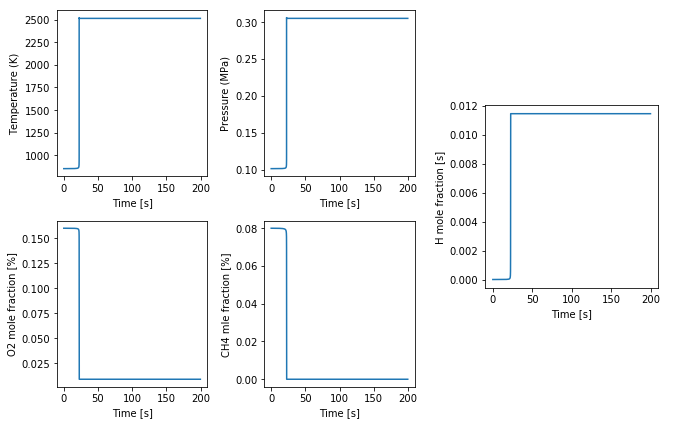
\includegraphics[width=0.5\textwidth]{example_data.png}
\caption{\label{fig:example}Example data .}
\end{figure}

\subsection{Using the 'airm' function}
The function '$airm$' defined earlier is used in three loops.
\subsubsection{The first loop}
In the first loop maximal pressures and temperatures are calculated as a function of $CH_4$ molar fractions,  with addition of 0, 1 and 2 moles of water, that is $water_mol$ is set as $0, 1$ and $2$. This coresponds to $0\%, 15.97\%$ and $27.54\%$ of $H_2O$ in the mixture (volumetric). $CH_4$ range tested is from 0 to 2 moles, in 41 iterations with an increase of $0.05$ moles each.
\begin{lstlisting}[language=python]
lp=41 #number of iterations for 1st loop
#preparing space for data
pdata = np.zeros((lp,3)) #without water
ch4m_data = np.zeros(lp) #without water
ch4m_w_data = np.zeros(lp) #with water
ch4m_2w_data = np.zeros(lp) #with water
pdata_w = np.zeros((lp,3)) #with 1 mol of water
pdata_2w = np.zeros((lp,3)) #with 2 moles of water
o2=1 
n2=0.78/0.21
ar=0.01/0.21
wt=1 #mole fraction of water in mixture
#in this loop CH4 mole fraction is changing from 0 to lp*i/2, with and without addition of water
for i in range(lp):
    pdata[i,:]=airm(temp=850, pressure=ct.one_atm, water_mol=0, ch4_mol=i/2, plot=0) #without water
    pdata_w[i,:]=airm(temp=850, pressure=ct.one_atm, water_mol=wt, ch4_mol=i/2, plot=0) #with water
    pdata_2w[i,:]=airm(temp=850, pressure=ct.one_atm, water_mol=2*wt, ch4_mol=i/2, plot=0) #with water
    ch4m_data[i]=(i/20)/(i/20+o2+n2+ar)*100      #molar/volume fraction of CH4 in mixture, when there is no water
    ch4m_w_data[i]=(i/20)/(i/20+o2+n2+ar+wt)*100 #molar/volume fraction of CH4 in mixture, when there is 1 mole water
    ch4m_2w_data[i]=(i/20)/(i/20+o2+n2+ar+2*wt)*100 #molar/volume fraction of CH4 in mixture, when there are 2 moles of water
\end{lstlisting}
\subsubsection{The second loop}
In the second loop maximal pressures and temperatures are calculated as a function of initial temperatures. The range of temperatures tested is $850-2100\ K$, in 26 iterations with an increase of $50\ K$ in each. The $CH_4$ fraction is constant, equal to $0.5\ moles$.
\begin{lstlisting}[language=python]
l2p=26 #number of iterations for 2nd loop
#preparing space for data
pdata2 = np.zeros((l2p,3)) #without water
pdata2_w = np.zeros((l2p,3)) #with 1 moles of water
pdata2_2w = np.zeros((l2p,3)) #with 2 moles of  water
temps = np.zeros(l2p)
#loop through initial temperatures
for j in range(l2p):
    current_temp=850+j*50
    pdata2[j,:]=airm(temp=current_temp, pressure=ct.one_atm, water_mol=0, ch4_mol=5, plot=0)
    pdata2_w[j,:]=airm(temp=current_temp, pressure=ct.one_atm, water_mol=wt, ch4_mol=5, plot=0)
    pdata2_2w[j,:]=airm(temp=current_temp, pressure=ct.one_atm, water_mol=2*wt, ch4_mol=5, plot=0)
    temps[j]=current_temp
\end{lstlisting}

\subsubsection{The third loop}
In the third loop maximal pressures and temperatures are calculated as a function of initial pressures. The range of pressures tested is $0.5-25.5\ atm\ (0.051-2.584 MPa)$, in 26 iterations with an increase of $0.5\ atm\ (0.101325\ MPa)$ in each. The $CH_4$ fraction is constant, equal to $0.5\ moles$.
\begin{lstlisting}[language=python]
l3p=26 #number of loop iterations
#preparing space for data
pdata3 = np.zeros((l3p,3)) #without water
pdata3_w = np.zeros((l3p,3)) #with 1 mole of water
pdata3_2w = np.zeros((l3p,3)) #with 2 moles of water
press = np.zeros(l3p)
#wt=1 #mole fraction of water in mixture
#loop through start pressures
for j in range(l3p):
    current_press=(0.5*ct.one_atm)+ct.one_atm*j #current start pressure in [Pa]
    pdata3[j,:]=airm(temp=850, pressure=current_press, water_mol=0, ch4_mol=5, plot=0)
    pdata3_w[j,:]=airm(temp=850, pressure=current_press, water_mol=wt, ch4_mol=5, plot=0)
    pdata3_2w[j,:]=airm(temp=850, pressure=current_press, water_mol=2*wt, ch4_mol=5, plot=0)
    press[j]=current_press #in [Pa]
\end{lstlisting}

\subsection{Plotting and saving the data}
\subsubsection{The first loop}
Data acquired in the first loop is then plotted:
\begin{lstlisting}[language=python]
plt.clf()
plt.figure(figsize=(20,20)) #setting size of figures
#w/o water
plt.subplot(2, 2, 1)
plt.plot(ch4m_data, pdata[:,1]/1.e+6, label='without water')
plt.xlabel('CH4 (%vol)')
plt.ylabel('P_max [Mpa]')
plt.subplot(2, 2, 2)
plt.plot(ch4m_data, pdata[:,0], label='without water')
plt.xlabel('CH4 (%vol)')
plt.ylabel('T_max [K]')
#with 1 mole of water
plt.subplot(2, 2, 1)
plt.plot(ch4m_w_data, pdata_w[:,1]/1.e+6, label='15.97% of water')
plt.xlabel('CH4 (%vol)')
plt.ylabel('P_max [Mpa]')
plt.subplot(2, 2, 2)
plt.plot(ch4m_data, pdata_w[:,0], label='15.97% of water')
plt.xlabel('CH4 (%vol)')
plt.ylabel('T_max [K]')
#with 2 moles of water
plt.subplot(2, 2, 1)
plt.plot(ch4m_2w_data, pdata_2w[:,1]/1.e+6, label='27.54% of water')
plt.xlabel('CH4 (%vol)')
plt.ylabel('P_max [Mpa]')
plt.legend()
plt.subplot(2, 2, 2)
plt.plot(ch4m_data, pdata_2w[:,0], label='27.54% of water')
plt.xlabel('CH4 (%vol)')
plt.ylabel('T_max [K]')
plt.legend()
plt.tight_layout()
plt.show()

plt.clf()
plt.figure(figsize=(10,10))
plt.subplot(1, 1, 1)
plt.plot(ch4m_data, pdata[:,3]*1.e+3, label='without water')
plt.xlabel('CH4 (%vol)')
plt.ylabel('Autoign delay [ms]')
plt.subplot(1, 1, 1)
plt.plot(ch4m_data, pdata_w[:,3]*1.e+3, label='15.97% of water')
plt.xlabel('CH4 (%vol)')
plt.ylabel('Autoign delay [ms]')
plt.subplot(1, 1, 1)
plt.plot(ch4m_data, pdata_2w[:,3]*1.e+3, label='27.54% of water')
plt.xlabel('CH4 (%vol)')
plt.ylabel('Autoign delay [ms]')
plt.legend()
plt.grid()
plt.tight_layout()
plt.show()

csv_file = 'graphdata.csv'
with open(csv_file, 'w') as outfile:
    writer = csv.writer(outfile)
    writer.writerow(['The first loop'])
    writer.writerow(['Without water'])
    writer.writerow(['CH4 [%]', 'Tmax [K]', 'Pmax [MPa]', 'dP/dt max [MPa/s]', 'adt [s]'])
    for i in range(lp):
         writer.writerow([ch4m_data[i], pdata[i,0], pdata[i,1]/1.e+6, pdata[i,2], pdata[i,3]])
    writer.writerow(['With 1 mole of water'])
    writer.writerow(['CH4[%]', 'Tmax [K]', 'Pmax [MPa]', 'dP/dt max [MPa/s]', 'adt [s]'])
    for i in range(lp):
         writer.writerow([ch4m_w_data[i], pdata_w[i,0], pdata_w[i,1]/1.e+6, pdata_w[i,2], pdata_w[i,3]])
    writer.writerow(['With 2 moles of water'])
    writer.writerow(['CH4[%]', 'Tmax [K]', 'Pmax [MPa]', 'dP/dt max [MPa/s]', 'adt [s]'])
    for i in range(lp):
         writer.writerow([ch4m_2w_data[i], pdata_2w[i,0], pdata_2w[i,1]/1.e+6, pdata_2w[i,2],  pdata_2w[i,3]])
\end{lstlisting}
\subsubsection{The second loop}
Data acquired in the second loop is then plotted:
\begin{lstlisting}[language=python]
plt.clf()
plt.figure(figsize=(20,20))
#w/o water
l1=plt.subplot(2, 2, 1)
plt.plot(temps, pdata2[:,1]/1.e+6, label='without water')
plt.xlabel('Temperature [K]')
plt.ylabel('P_max [MPa]')
plt.subplot(2, 2, 2)
plt.plot(temps, pdata2[:,0], label='without water')
plt.xlabel('Temperature [K]')
plt.ylabel('T_max [K]')
#with water
plt.subplot(2, 2, 2)
plt.plot(temps, pdata2_w[:,0], label='15.97% of water')
plt.xlabel('Temperature [K]')
plt.ylabel('T_max [K]')
plt.subplot(2, 2, 1)
plt.plot(temps, pdata2_w[:,1]/1.e+6, label='15.97% of water')
plt.xlabel('Temperature [K]')
plt.ylabel('P_max [MPa]')
#with 2 moles of water
plt.subplot(2, 2, 2)
plt.plot(temps, pdata2_2w[:,0], label='27.54% of water')
plt.xlabel('Temperature [K]')
plt.ylabel('T_max [K]')
plt.legend()
plt.subplot(2, 2, 1)
plt.plot(temps, pdata2_2w[:,1]/1.e+6, label='27.54% of water')
plt.xlabel('Temperature [K]')
plt.ylabel('P_max [MPa]')
plt.legend()
plt.tight_layout()
plt.show()

plt.clf()
plt.figure(figsize=(10,10))
plt.subplot(1, 1, 1)
plt.plot(1000/temps, pdata2[:,3]*1.e+3, label='without water')
plt.xlabel('1000/T [1/K]')
plt.yscale('log')
plt.ylabel('Autoign delay [ms]')
plt.subplot(1, 1, 1)
plt.plot(1000/temps, pdata2_w[:,3]*1.e+3, label='15.97% of water')
plt.xlabel('1000/T [1/K]')
plt.yscale('log')
plt.ylabel('Autoign delay [ms]')
plt.subplot(1, 1, 1)
plt.plot(1000/temps, pdata2_2w[:,3]*1.e+3, label='27.54% of water')
plt.xlabel('1000/T [1/K]')
plt.yscale('log')
plt.ylabel('Autoign delay [ms]')
plt.legend()
plt.grid()
plt.tight_layout()
plt.show()

csv_file = 'graphdata.csv'
with open(csv_file, 'a') as outfile:
    writer = csv.writer(outfile)
    writer.writerow(['The second loopr'])
    writer.writerow(['Without water'])
    writer.writerow(['T0 [K]', 'Tmax [K]', 'Pmax [MPa]', 'dP/dt max [MPa/s]', 'adt [s]'])
    for i in range(l2p):
         writer.writerow([temps[i], pdata2[i,0], pdata2[i,1]/1.e+6, pdata2[i,2], pdata2[i,3]])
    writer.writerow(['With 1 mole of water'])
    writer.writerow(['T0 [K]', 'Tmax [K]', 'Pmax [MPa]', 'dP/dt max [MPa/s]', 'adt [s]'])
    for i in range(l2p):
         writer.writerow([temps[i], pdata2_w[i,0], pdata2_w[i,1]/1.e+6, pdata2_w[i,2], pdata2_w[i,3]])
    writer.writerow(['With 2 moles of water'])
    writer.writerow(['T0 [K]', 'Tmax [K]', 'Pmax [MPa]', 'dP/dt max [MPa/s]', 'adt [s]'])
    for i in range(l2p):
         writer.writerow([temps[i], pdata2_2w[i,0], pdata2_2w[i,1]/1.e+6, pdata2_2w[i,2], pdata2_2w[i,3]])
\end{lstlisting}
\subsubsection{The third loop}
Data acquired in the third loop is then plotted:
\begin{lstlisting}[language=python]
plt.clf() #clear the current figure
#w/o water
plt.figure(figsize=(20,20))
plt.subplot(2, 2, 1)
plt.plot(press/1.e+6, pdata3[:,1]/1.e+6, label='without of water')
plt.xlabel('Pressure [MPa]')
plt.ylabel('P_max [MPa]')
plt.subplot(2, 2, 2)
plt.plot(press/1.e+6, pdata3[:,0], label='without of water')
plt.xlabel('Pressure [MPa]')
plt.ylabel('T_max [K]')
#with 1 mole of water
plt.subplot(2, 2, 1)
plt.plot(press/1.e+6, pdata3_w[:,1]/1.e+6, label='15.97% of water')
plt.xlabel('Pressure [MPa]')
plt.ylabel('P_max [MPa]')
plt.subplot(2, 2, 2)
plt.plot(press/1.e+6, pdata3_w[:,0], label='15.97% of water')
plt.xlabel('Pressure [MPa]')
plt.ylabel('T_max [K]')
#with 2 moles of water
plt.subplot(2, 2, 1)
plt.plot(press/1.e+6, pdata3_2w[:,1]/1.e+6, label='27.54% of water')
plt.xlabel('Pressure [MPa]')
plt.ylabel('P_max [MPa]')
plt.legend()
plt.subplot(2, 2, 2)
plt.plot(press/1.e+6, pdata3_2w[:,0], label='27.54% of water')
plt.xlabel('Pressure [MPa]')
plt.ylabel('T_max [K]')
plt.legend()
plt.tight_layout()
plt.show()       

plt.clf()
plt.figure(figsize=(10,10))
plt.subplot(1, 1, 1)
plt.plot(press/1.e+6, pdata3[:,3]*1.e+3, label='without water')
plt.xlabel('Pressure [MPa]')
plt.ylabel('Autoign delay [ms]')
plt.subplot(1, 1, 1)
plt.plot(press/1.e+6, pdata3_w[:,3]*1.e+3, label='15.97% of water')
plt.xlabel('Pressure [MPa]')
plt.ylabel('Autoign delay [ms]')
plt.subplot(1, 1, 1)
plt.plot(press/1.e+6, pdata3_2w[:,3]*1.e+3, label='27.54% of water')
plt.xlabel('Pressure [MPa]')
plt.yscale('log')
plt.ylabel('Autoign delay [ms]')
plt.legend()
plt.tight_layout()
plt.show()       

csv_file = 'graphdata.csv'
with open(csv_file, 'a') as outfile:
    writer = csv.writer(outfile)
    writer.writerow(['The third loop'])
    writer.writerow(['Without water'])
    writer.writerow(['p0 [MPa]', 'Tmax [K]', 'Pmax [MPa]', 'dP/dt max [MPa/s]', 'adt [s]'])
    for i in range(l3p):
         writer.writerow([press[i]/1.e+6, pdata3[i,0], pdata3[i,1]/1.e+6, pdata3[i,2], pdata3[i,3]])
    writer.writerow(['With 1 mole of water'])
    writer.writerow(['p0 [MPa]', 'Tmax [K]', 'Pmax [MPa]', 'dP/dt max [MPa/s]', 'adt [s]'])
    for i in range(l3p):
         writer.writerow([press[i]/1.e+6, pdata3_w[i,0], pdata3_w[i,1]/1.e+6, pdata3_w[i,2], pdata3_w[i,3]])
    writer.writerow(['With 2 moles of water'])
    writer.writerow(['p0 [MPa]', 'Tmax [K]', 'Pmax [MPa]', 'dP/dt max [MPa/s]', 'adt [s]'])
    for i in range(l3p):
         writer.writerow([press[i]/1.e+6, pdata3_2w[i,0], pdata3_2w[i,1]/1.e+6, pdata3_2w[i,2], pdata3_2w[i,3]])
\end{lstlisting}

\section{Results}
\subsection{Results from the first loop}
Maximal explosion pressure is highest for $12\%$ of $CH_4$ in the mixture when there is no water, for $9.43\%$ when there is 1 mole of water and for $7.52$ when there are 2 moles of water. The maximal pressure is getting lower the more water is in the mixture and occurs at lower fraction of methane.
Those results were compared to those acquired by Shen et al.\cite{shen2016explosion}, but because of Cantera's zero dimensionality, spark ignition couldn't been simulated, thus minimal temperature tested was $850 K$ in comparison to $298\ K$ in aforementioned paper.
In Cantera simulation, maximal pressure without addition of water was determined to occur at higher vol. fraction of $CH_4$ (12\% vs 10.5\%) than in experiment. The maximal pressure was $0.2461\ MPa$, which is 3.33 times lower than in Shen's experiment. Like in Shen's experiment, the point of maximal pressure was moving towards lower $CH_4$ vol. fractions when water was added and was lower with water than than when there was no water added.
The discrepancy in results may be due to different phenomenons tested, that is ignition instead of autoignition.
Figure \ref{fig:1} shows comparison of acquired maximal pressures as a function of methane vol. fraction in the mixture.
\begin{figure}[H]
    \centering
    \begin{subfigure}[b]{0.4\textwidth}
        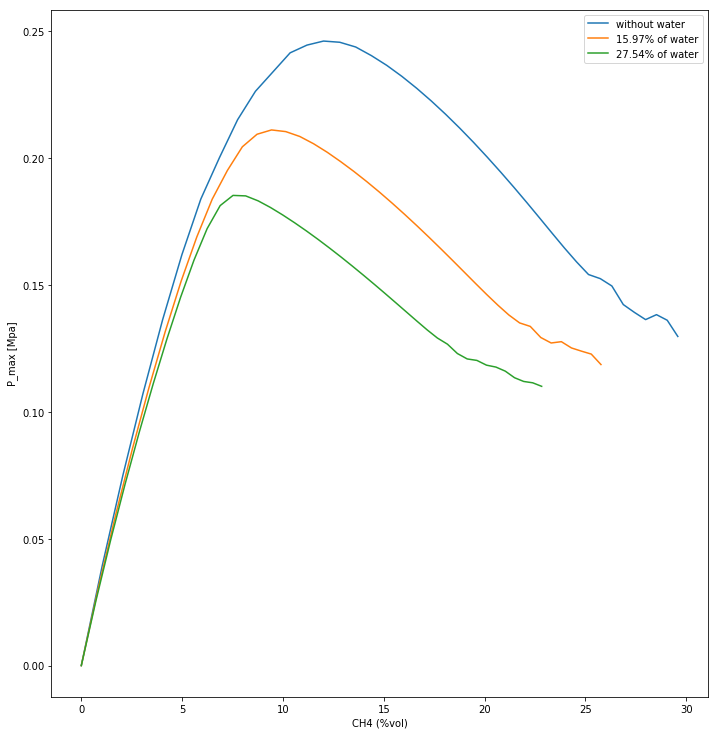
\includegraphics[width=\textwidth]{1_Pmax_to_CH4_2.png}
        	\caption{Max. explosion pressure as a function of methane fraction computed in Cantera}
        \label{fig:1_1a}
    \end{subfigure}
    \qquad
    \begin{subfigure}[b]{0.5\textwidth}
        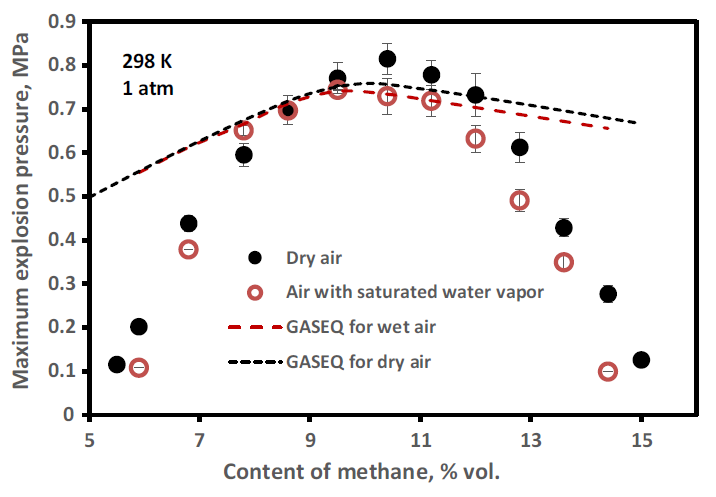
\includegraphics[width=\textwidth]{f1_a2.png}
        	\caption{Max. temperature as a function of methane fraction from \cite{shen2016explosion}}
        \label{fig:1_1b}
    \end{subfigure}
    \caption{Results comparison}\label{fig:1}
\end{figure}
\begin{figure}[h!]
\centering
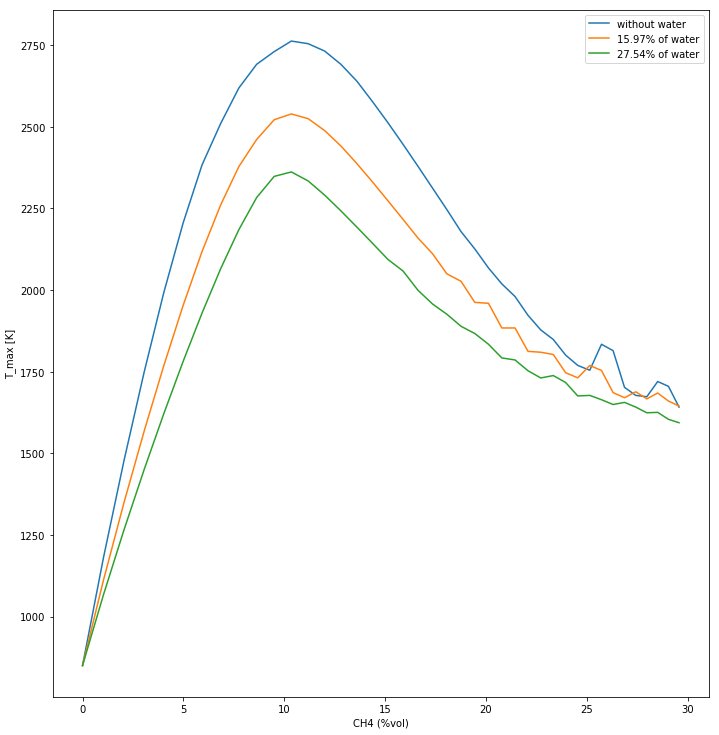
\includegraphics[width=0.5\textwidth]{1_Tmax_to_CH4.png}
\caption{\label{fig:1_2}Maximum temperatures as a function of methane vol. fractions acquired in Cantera}
\end{figure}
\begin{figure}[H]
\centering
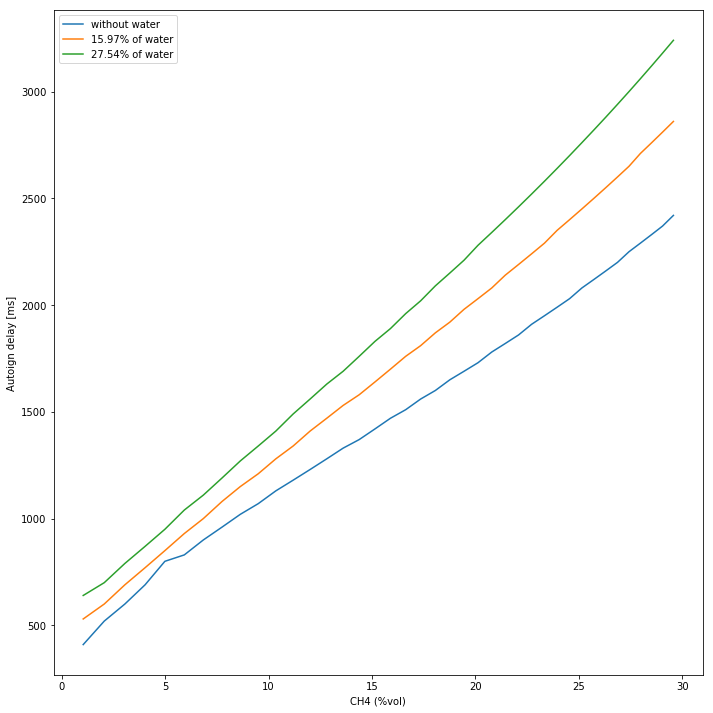
\includegraphics[width=0.5\textwidth]{1_adt_to_CH4.png}
\caption{\label{fig:1_3}Autoiginition delay times acquired in Cantera}
\end{figure}

\subsection{Results from the second loop}
Maximal explosion pressures are getting lower the higher the temperature. Without water the drop between 850 and 2100 degrees is $75\%$, with 15\% of water $76.6\%$ and $77.4\%$.
Maximal temperature is increasing with the increase of initial temperature. Relative maximal temperature for initial 850K is 1880 K and drops on average by 75.3K every 100K more for the initial temperature. The drop is 70.7/100 for 15.97\% of water and 65.1/100 for 27.64\% of water in the mixture (vol.).
Results are shown on Figures \ref{fig:2} and \ref{fig:2_3}.

\begin{figure}[H]
    \centering
    \begin{subfigure}[h]{0.4\textwidth}
        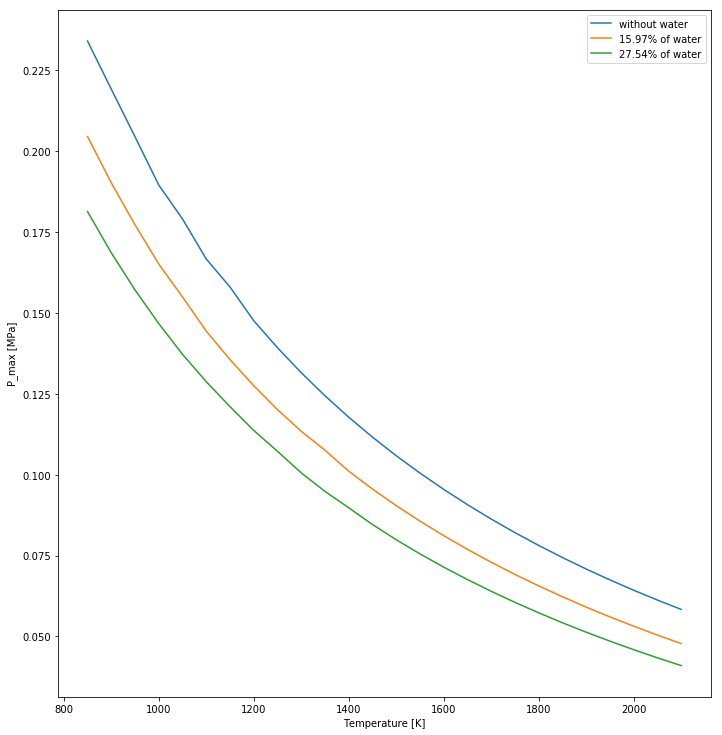
\includegraphics[width=\textwidth]{2_Pmax_to_T_2.png}
        	\caption{Max. explosion pressure as a function of initial temperature}
        \label{fig:2_1}
    \end{subfigure}
    \qquad
    \begin{subfigure}[h]{0.4\textwidth}
        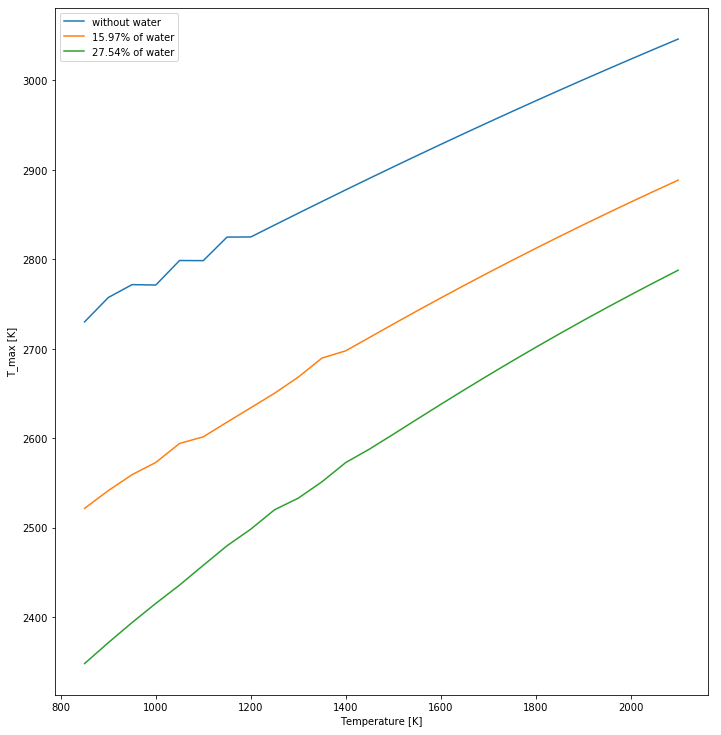
\includegraphics[width=\textwidth]{2_Tmax_to_T.png}
        	\caption{Max. temperature as a function of initial temperature}
        \label{fig:2_2}
    \end{subfigure}
    \caption{Results from the second loop}\label{fig:2}
\end{figure}
\begin{figure}[H]
\centering
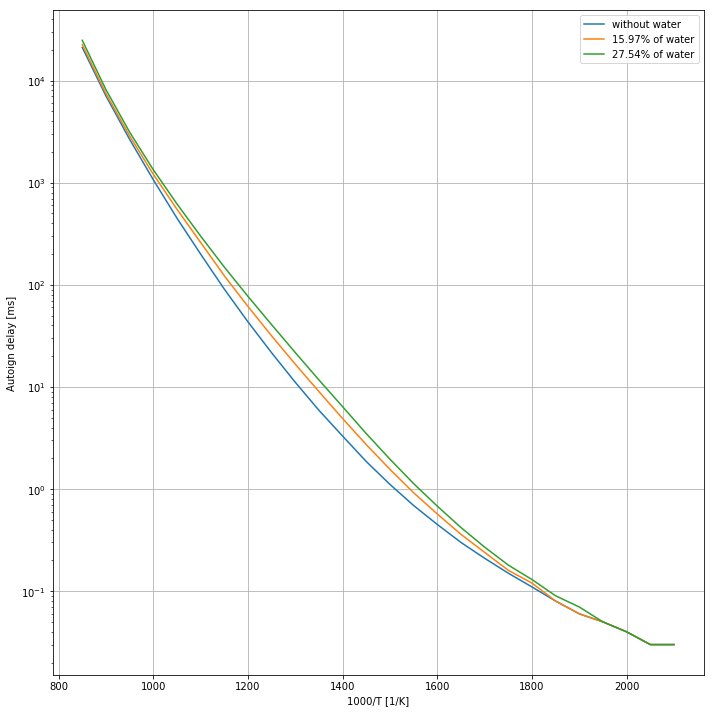
\includegraphics[width=0.75\textwidth]{2_adt_to_T_b.png}
\caption{\label{fig:2_3}Autoiginition delay times acquired in Cantera}
\end{figure}

Additional computations were performed for no water nad 8\% of water in the mixture (vol.) at the pressure of 10 atm to compare it to results reported by Goy et al.\cite{Goy2001}, they are shown together with Cantera results on Figure \ref{fig:2_goy}
\begin{figure}[H]
\centering
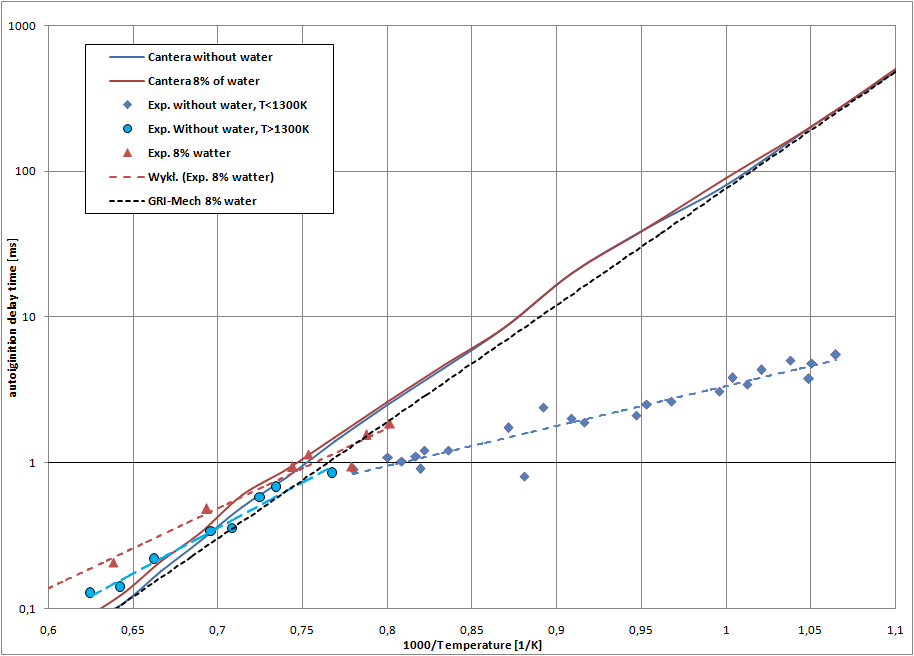
\includegraphics[width=0.75\textwidth]{2_whole_graph_slopes.png}
\caption{\label{fig:2_goy}Comarison of results from Cantera and \cite{Goy2001}}
\end{figure}
Data from Cantera simulation is fairly consistent (relative error of 4.84\% for 900K, 37\% for 1300K and 27\% for 1500K) with the data calculated using also GRI 3.0 mechanism from Goy paper, but diverges greatly from experimental data for temperatures below 1300K (small relative error of 34.5\% for 1500K, 27.86\% for 1300K and a massive error of 8581.3\% for 900K). Slopes for exponential trend lines for experimental data for temperatures below and above 1300K are different. This is because Version 3.0 of the GRI kinetic mechanism is validated only for temperatures above 1350 K.\cite{Goy2001}. Goy et al. states, that this may be due to change in activation energy at low temperature.

\subsection{Results from the third loop}
Maximal explosion pressure is changing linearly with initial pressure. The increase of 1MPa of initial pressure corresponds to increase of 1.886, 1.507 and 1.337 for no water, 15.67\% and 27.54\% of $CH_4$ fraction in the mixture (vol.) respectively (see Figure \ref{fig:3_1}).
Maximal temperature for initial pressure of 0.5 atm is 7.33\% lower for 15.67\% of water in the mixture and 13.37\% for 27.64\% if water in the mixture (vol.) than when there was no water added. For initial pressure of 25.5 atm maximal temperature is 9.71\% lower for 15.67\% of water in the mixture and 17.18\% for 27.64\% of water in the mixture (vol.) than hen there was no water added (see Figure \ref{fig:3_2}).

\begin{figure}[H]
    \centering
    \begin{subfigure}[h]{0.4\textwidth}
        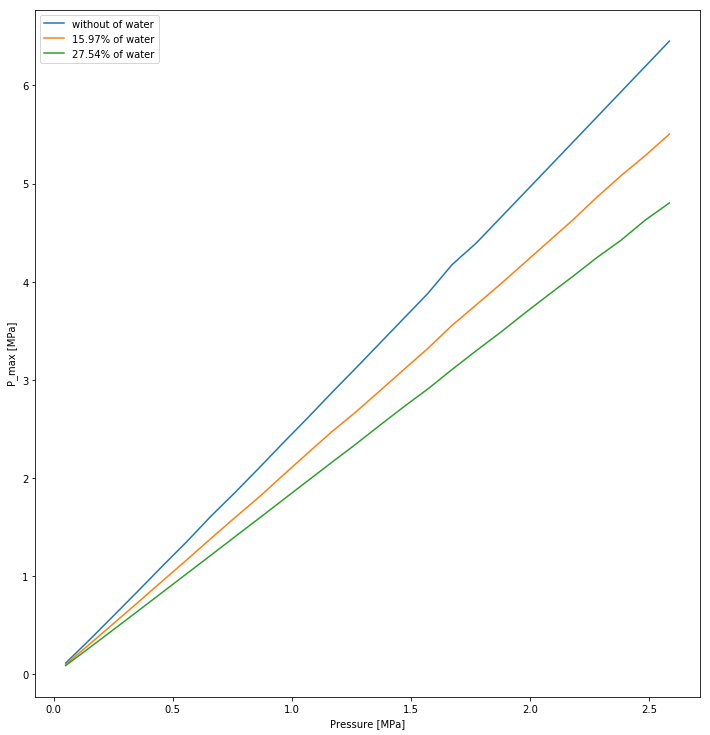
\includegraphics[width=\textwidth]{3_Pmax_to_P_2.png}
        	\caption{Max. explosion pressure as a function of initial pressure}
        \label{fig:3_1}
    \end{subfigure}
    \qquad
    \begin{subfigure}[h]{0.4\textwidth}
        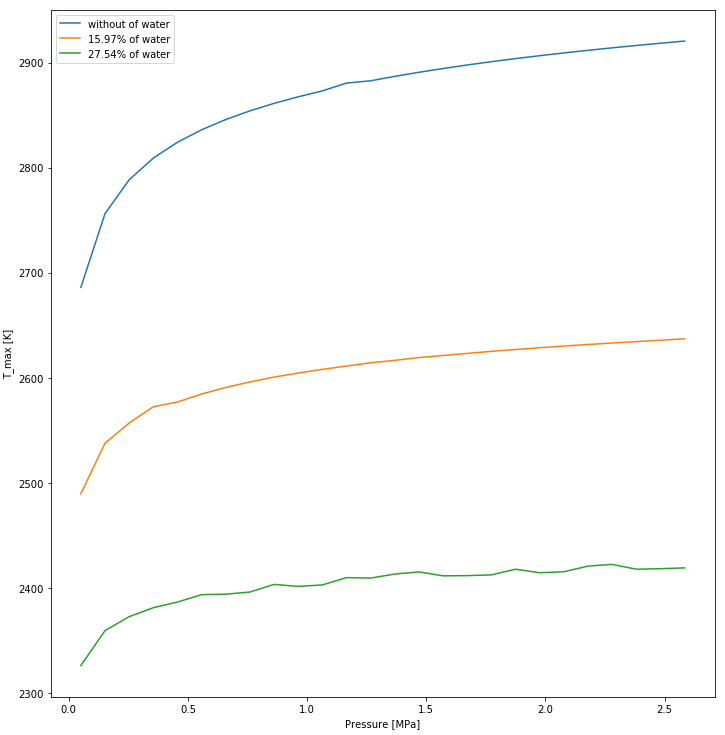
\includegraphics[width=\textwidth]{3_T_to_P_b.png}
        	\caption{Max. temperature as a function of initial pressure}
        \label{fig:3_2}
    \end{subfigure}
    \caption{Results from the third loop}\label{fig:3}
\end{figure}
\begin{figure}[H]
\centering
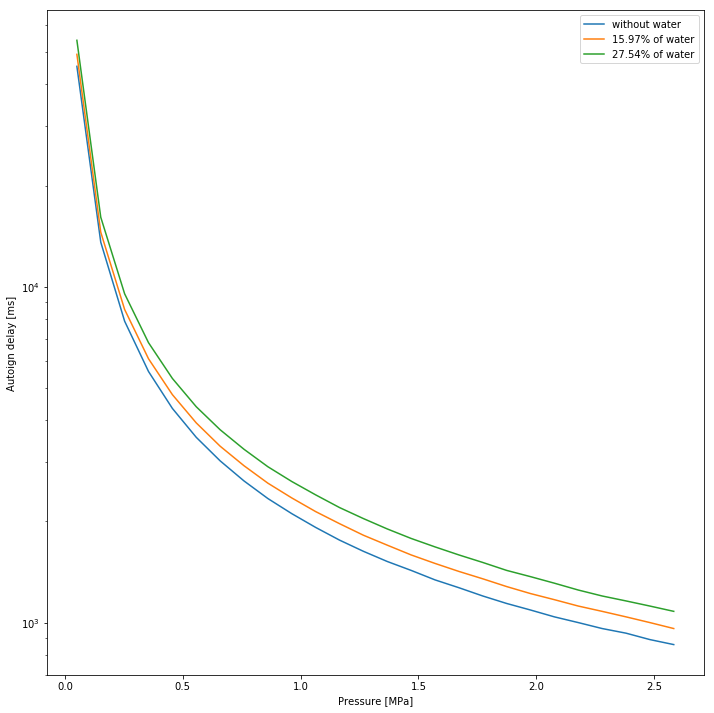
\includegraphics[width=0.5\textwidth]{3_adt_to_P.png}
\caption{\label{fig:3_3}Autoiginition delay times acquired in Cantera}
\end{figure}
\subsection{Maximal rate of pressure rise}
The maximal rate of pressure rise $(dP/dt)_(max)$ was calculated, but results were too far away from experimental data and varied greatly with the change time step, as seen on Figure \ref{fig:dPdt_timestep}. Because of that they were not analysed in this report.
\begin{figure}[H]
\centering
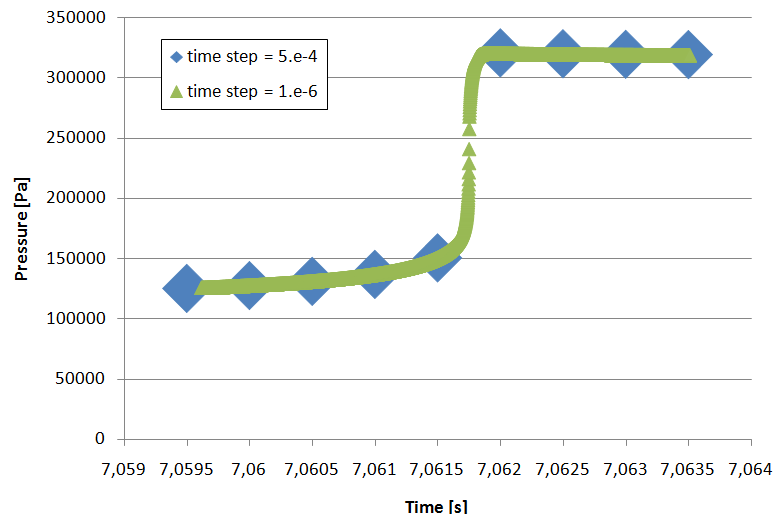
\includegraphics[width=0.5\textwidth]{press_time.PNG}
\caption{\label{fig:dPdt}Pressure as a function of time}
\end{figure}

\begin{figure}[H]
\centering
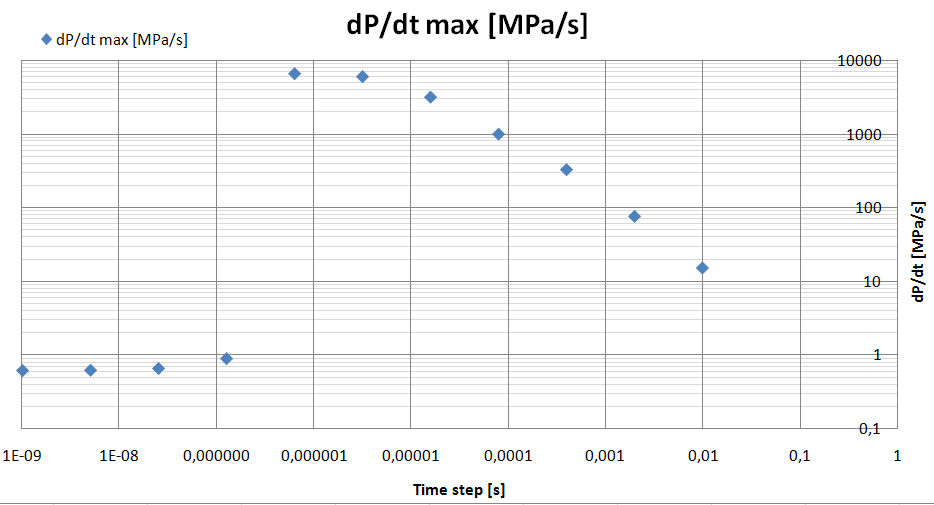
\includegraphics[width=0.5\textwidth]{dpdt_to_timestep.PNG}
\caption{\label{fig:dPdt_timestep}Maximal rate of pressure rise as a function of simulation time step}
\end{figure}


\subsection{Conclusions}
In each case addition of water vapour lowers maximal explosion pressure and maximal temperature, and also makes the autoignition delay time longer.

\bibliographystyle{plain}
\bibliography{ref}

\end{document}